\section{Addestramento su dataset aumentato}
Dopo aver ottenuto risultati significativi dal fine-tuning sul dataset filtrato, il passo successivo è stato individuare una serie di tecniche di augmentation da applicare al dataset. Per questo scopo, ho scelto di utilizzare la libreria Albumentations, che mi ha permesso di generare una versione aumentata del dataset. L'obiettivo era ampliare il subset di training e migliorare ulteriormente le prestazioni dei modelli.

\subsection{Albumentations}
Albumentations\cite{44} è una libreria open-source per l'augmentation delle immagini, progettata principalmente per il deep learning e l'addestramento di modelli di intelligenza artificiale. Essa offre un'ampia gamma di trasformazioni per le immagini, permettendo agli sviluppatori di migliorare la diversità dei dati di addestramento senza modificare manualmente le immagini originali. Le trasformazioni supportate includono modifiche di colore, traslazioni, rotazioni, crop, cambiamenti prospettici, aggiunta di rumore e molto altro ancora. Albumentations è particolarmente apprezzata per la sua velocità e flessibilità, essendo ottimizzata per gestire grandi quantità di dati e integrarsi senza problemi con framework di deep learning come PyTorch e TensorFlow. Nel nostro caso la libreria è stata utilizzata per generare direttamente tramite uno script nuovi dataset aumentati.

\newpage

\subsection{Prima Data Augmentation}

\subsubsection{Primo dataset aumentato}
Ho fatto un primo tentativo di data augmentation sul dataset filtrato, andando a generare una versione "augmented" di ciascuna immagine presente in \texttt{filtered-data/images/train}. Questo è stato fatto tramite uno script Python che applica le seguenti trasformazioni di Albumentations ad ogni immagine: 

\begin{figure}[ht]
    \centering
    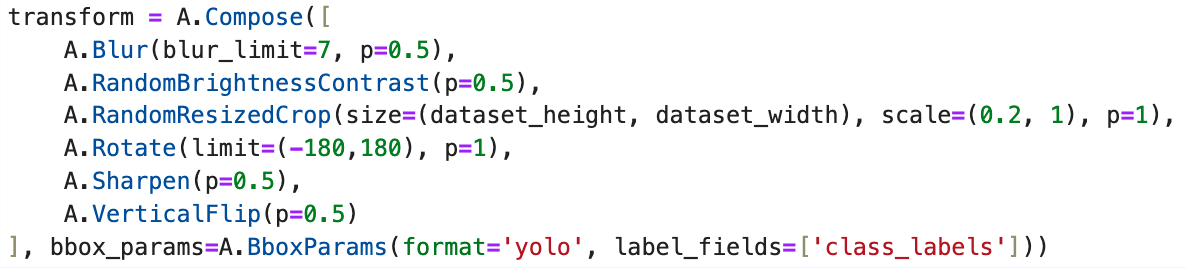
\includegraphics[width=0.9\textwidth]{files/capitoli/4-sperimentazione-risultati/assets/transform-1.png}
    \caption{\label{fig:transform-1}Definizione della trasformazione di Albumentations da applicare alle immagini}
\end{figure}

Il metodo \texttt{transform} di Albumentations consente l'applicazione di un insieme specifico di trasformazioni su un'immagine, gestendo probabilità e intervalli definiti. Questo processo genera una nuova immagine trasformata con relative annotazioni aggiornate, poiché le coordinate delle bounding box possono variare o essere rimosse a seguito delle trasformazioni.
A questo punto, le nuove immagini e annotazioni vengono utilizzate per creare il nuovo dataset aumentato \texttt{augmented-data-1}, il quale avrà esattamente il doppio degli esempi nel subset di training rispetto a \texttt{filtered-data}: 10.742 immagini del dataset originale e 10.742 immagini trasformate.
I subset val e test rimangono invariati.

\clearpage

\begin{figure}[ht]
    \centering
    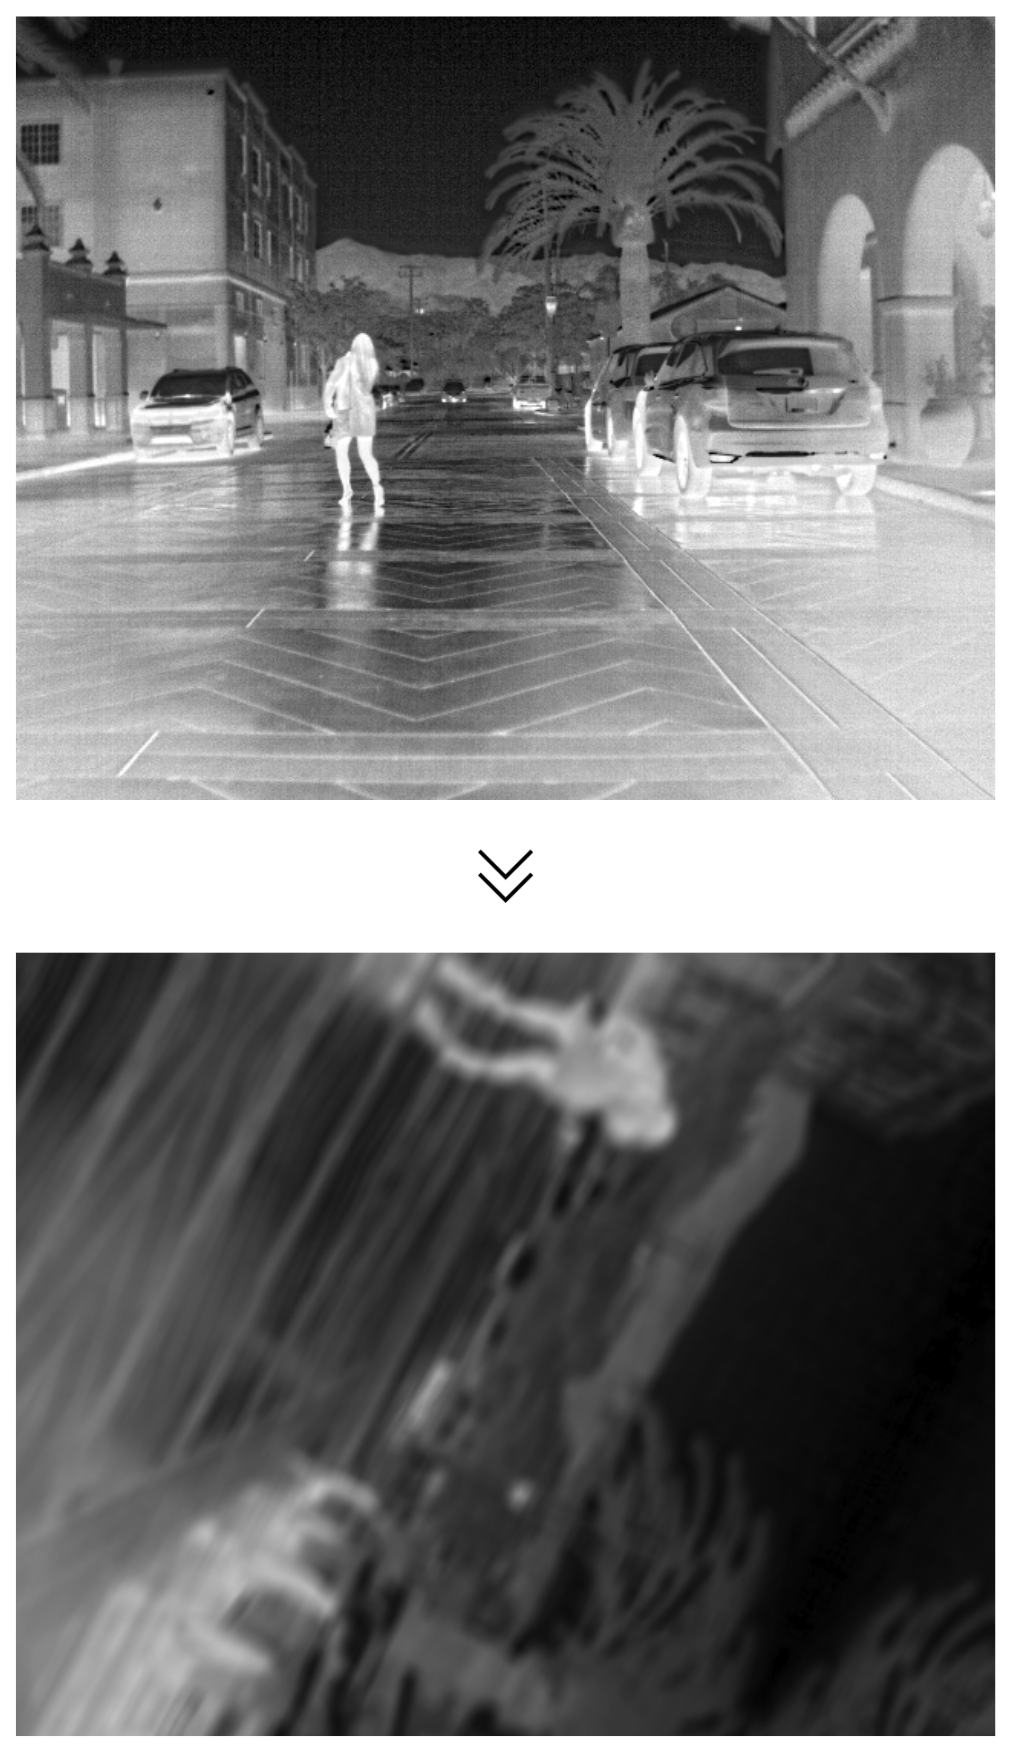
\includegraphics[width=0.8\textwidth]{files/capitoli/4-sperimentazione-risultati/assets/augmented-data-1-example.png}
    \caption{\label{fig:augmented-data-1-example}Esempio di immagine trasformata con la prima data augmentation}
\end{figure}

\clearpage

\subsubsection{Test modelli addestrati sul primo dataset aumentato}
Il secondo addestramento dei modelli è stato quindi condotto sul dataset \texttt{augmented-data-1}, mantenendo le stesse condizioni del primo, con 50 epochs e un batch size di 8.
I successivi test hanno prodotto i seguenti risultati:

\begin{figure}[ht]
    \centering
    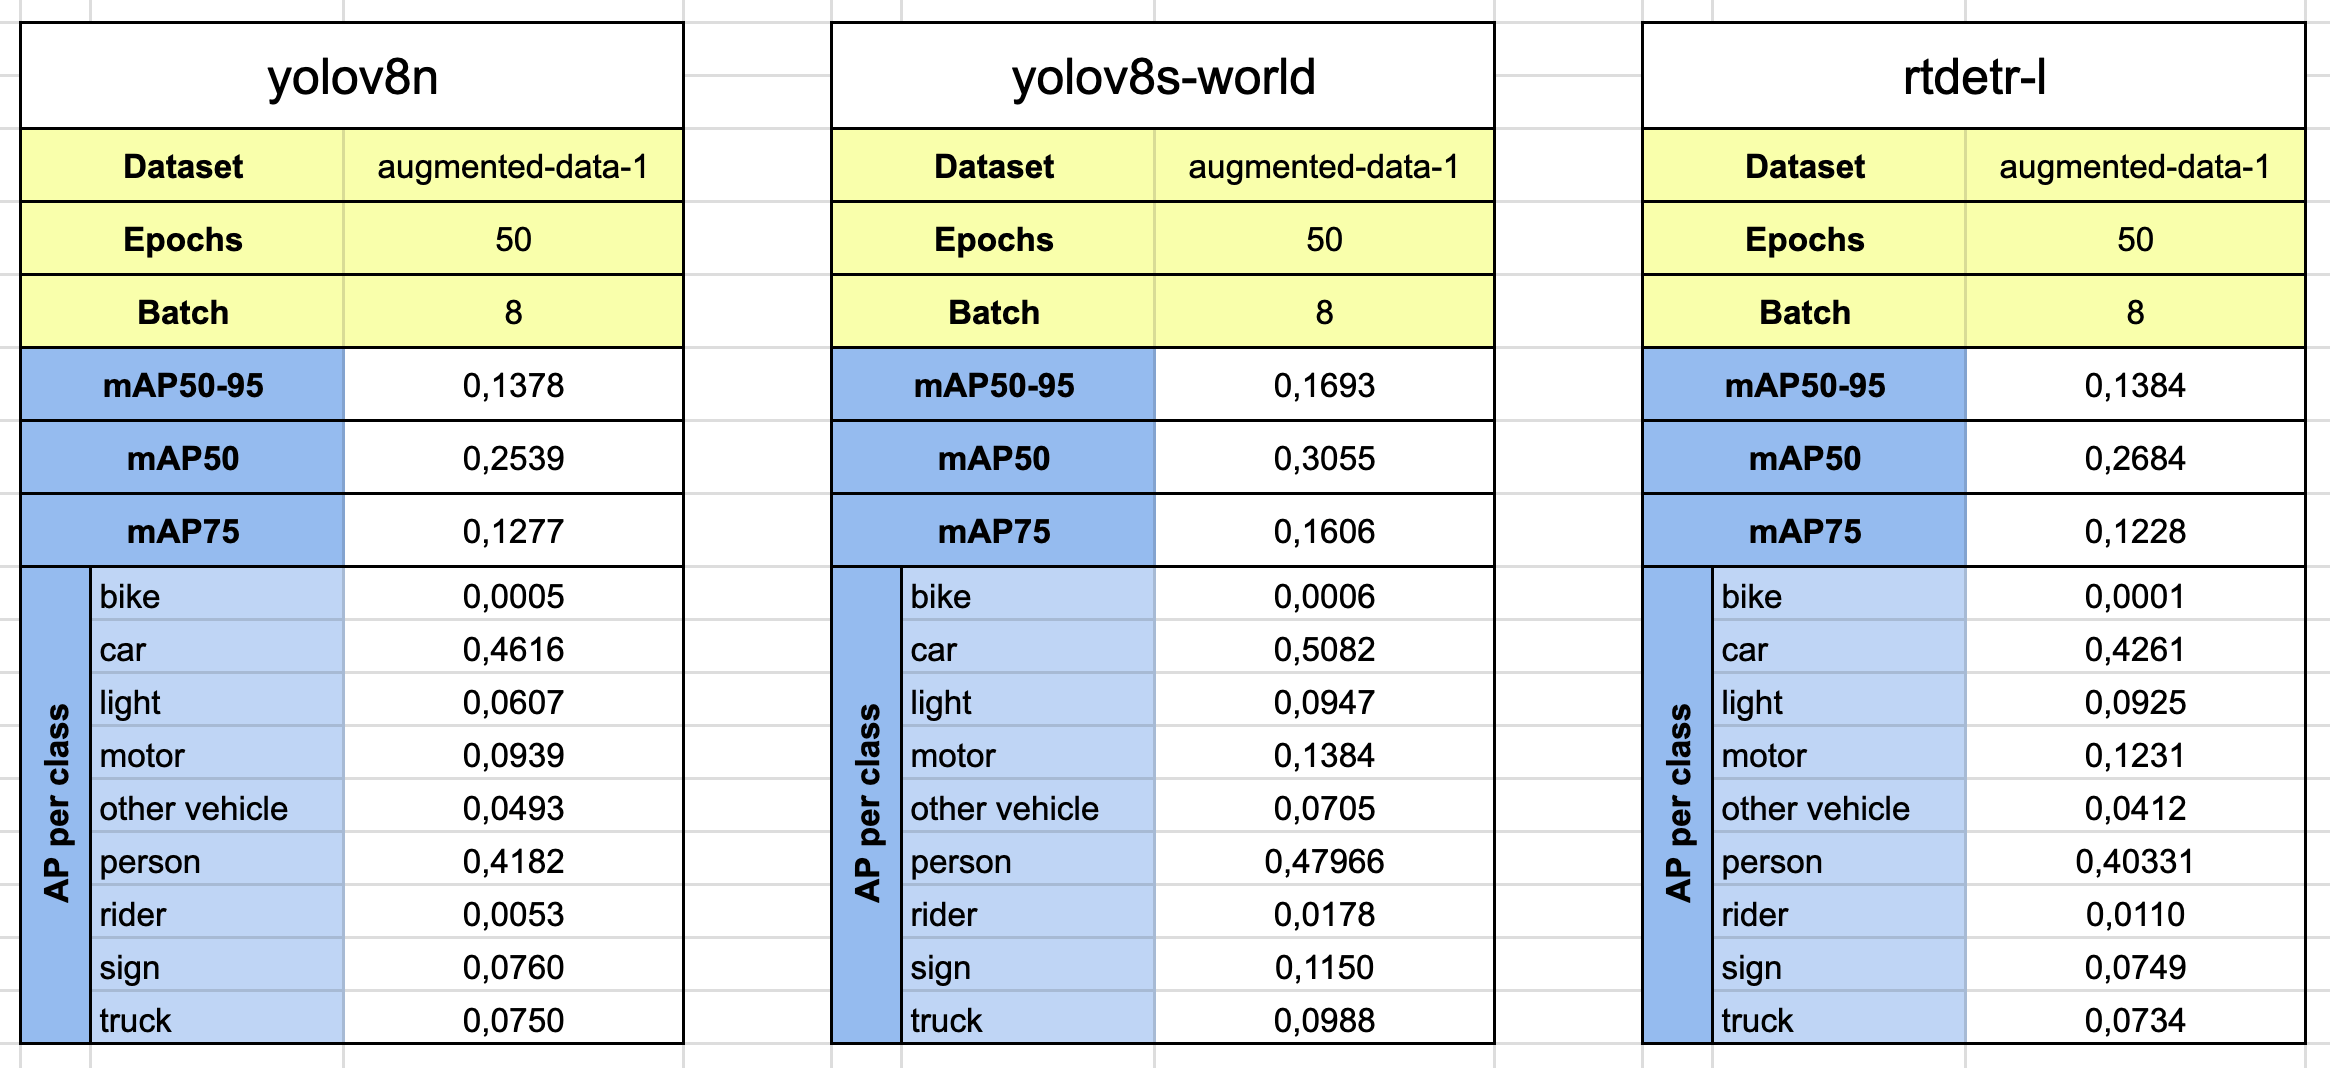
\includegraphics[width=1\textwidth]{files/capitoli/4-sperimentazione-risultati/assets/augmented-data-1-metrics.png}
    \caption{\label{fig:augmented-data-1-metrics}Risultati test dei modelli addestrati sul primo dataset aumentato}
\end{figure}

Notiamo che tutte le metriche, ad eccezione della mAP50-90 di YOLO-World, sono peggiorate con l'addestramento sul dataset aumentato; da questo evinciamo che la combinazione di trasformazioni utilizzate come augmentations è stata inefficace. Ciò è dovuto al fatto che alcune o tutte le trasformazioni erano inadeguate per il contesto delle immagini termiche: potrebbero aver modificato eccessivamente l'immagine o applicato trasformazioni incoerenti rispetto al dataset originario, come il Vertical Flip o la Rotation con un range di 180 gradi, compromettendo il "significato" delle immagini (ad esempio ribaltando macchine o altri elementi stradali, cosa che non accade nei dati catturati dalle termocamere).

\clearpage

\begin{figure}[ht]
    \centering
    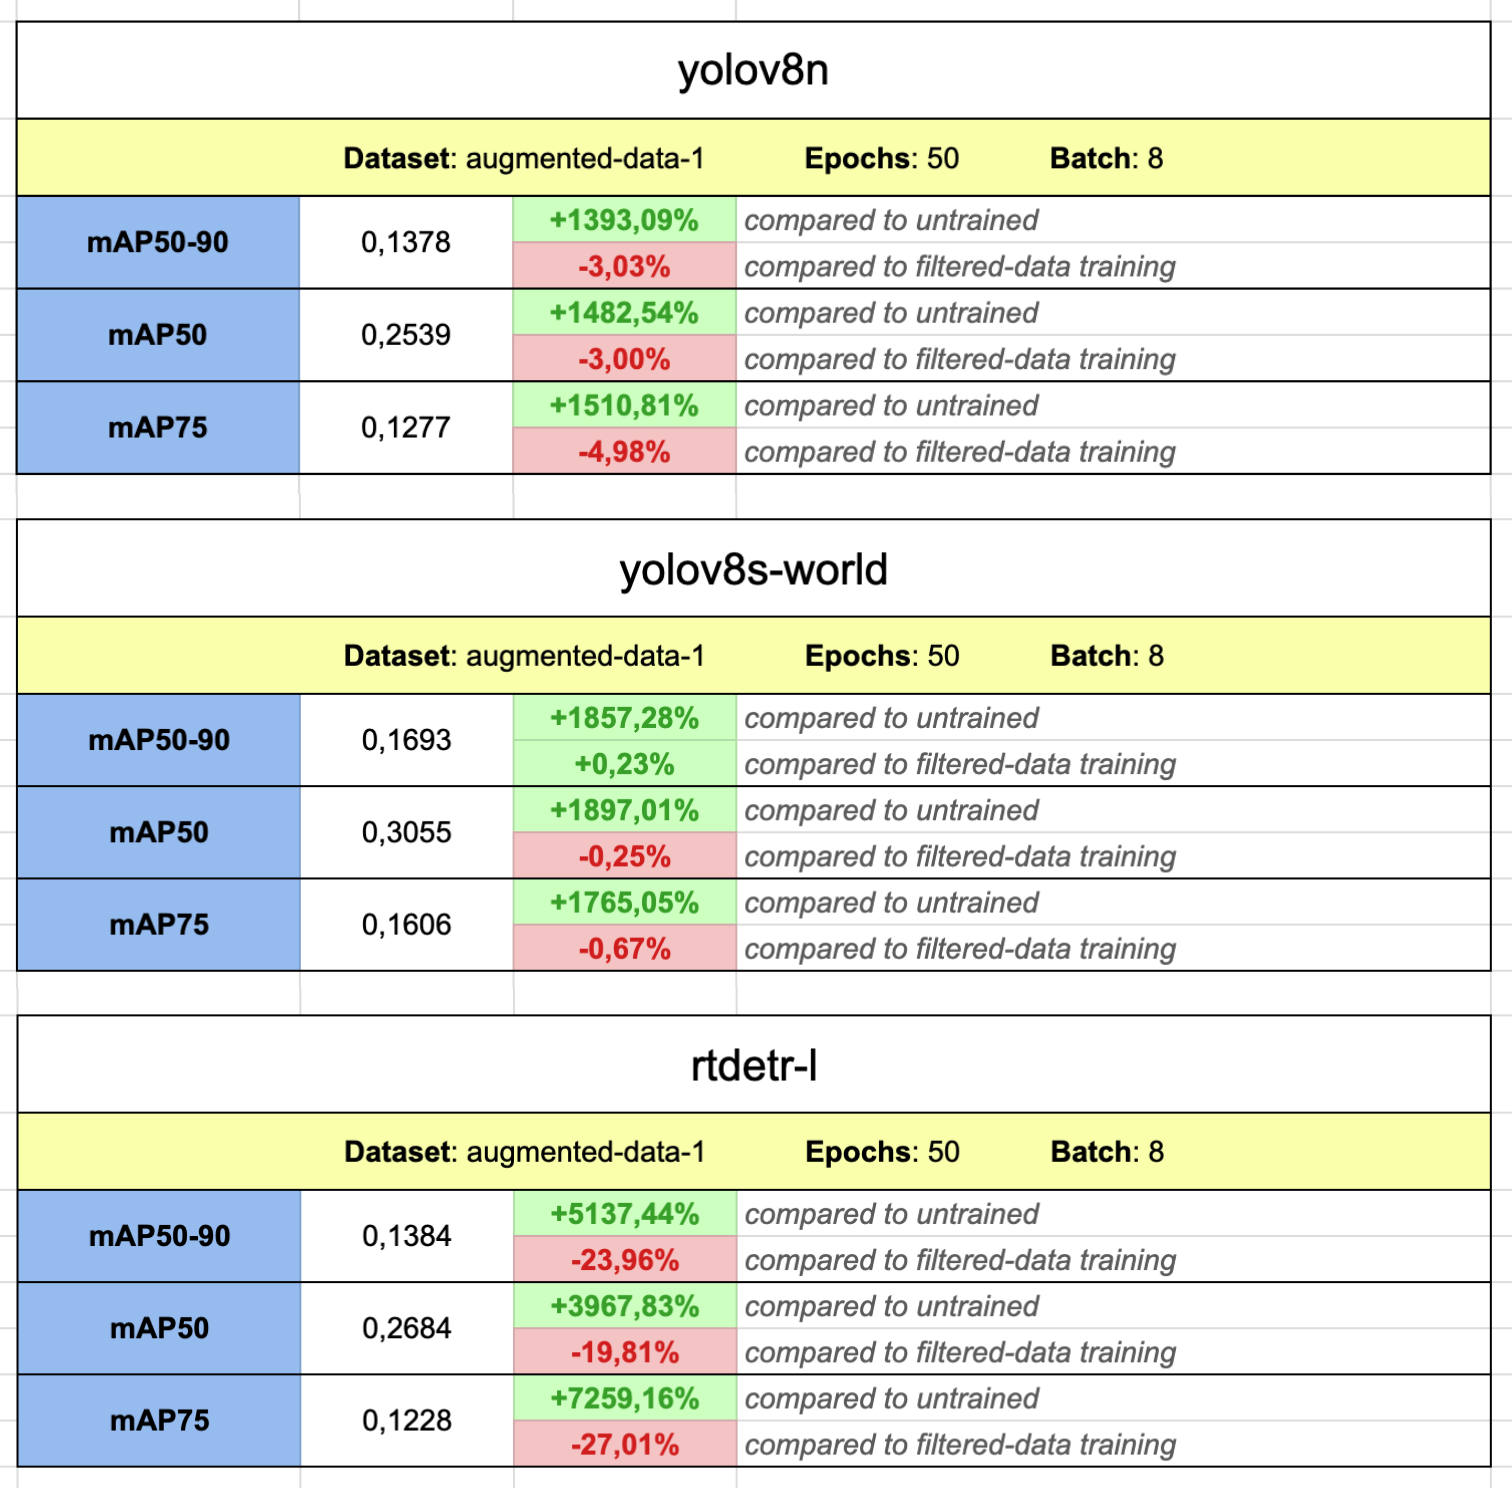
\includegraphics[width=0.9\textwidth]{files/capitoli/4-sperimentazione-risultati/assets/augmented-data-1-compare.png}
    \caption{\label{fig:augmented-data-1-compare}Confronto tra i risultati dei test dei modelli addestrati sul primo dataset aumentato e quelli dei precedenti test}
\end{figure}

\clearpage

\begin{figure}[ht]
    \centering
    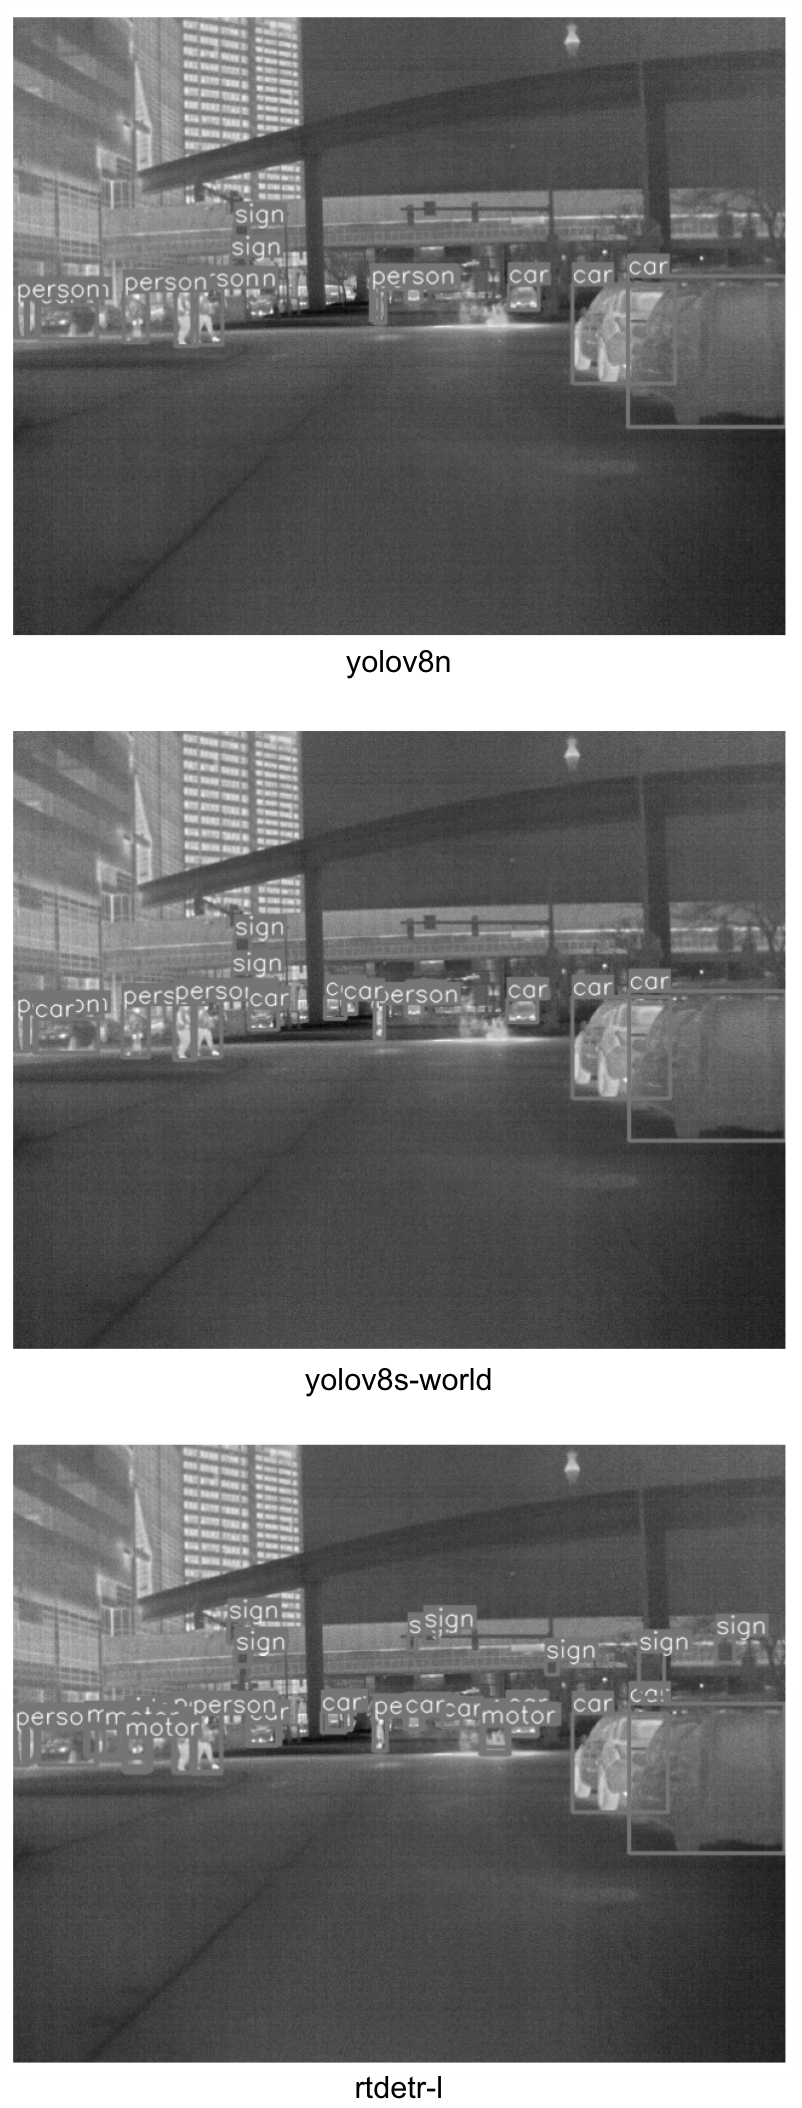
\includegraphics[width=0.6\textwidth]{files/capitoli/4-sperimentazione-risultati/assets/augmented-data-1-detections.png}
    \caption{\label{fig:augmented-data-1-detections}Detections effettutate dai modelli addestrati sul primo dataset aumentato}
\end{figure}

\clearpage

\subsection{Seconda Data Augmentation}

\subsubsection{Secondo dataset aumentato}
Visto il peggioramento delle prestazioni a seguito della prima data augmentation, sono andato a generare un secondo dataset aumentato tramite una nuova combinazione di trasformazioni mirata ad essere più coerente con il contesto delle immagini termiche:

\begin{figure}[ht]
    \centering
    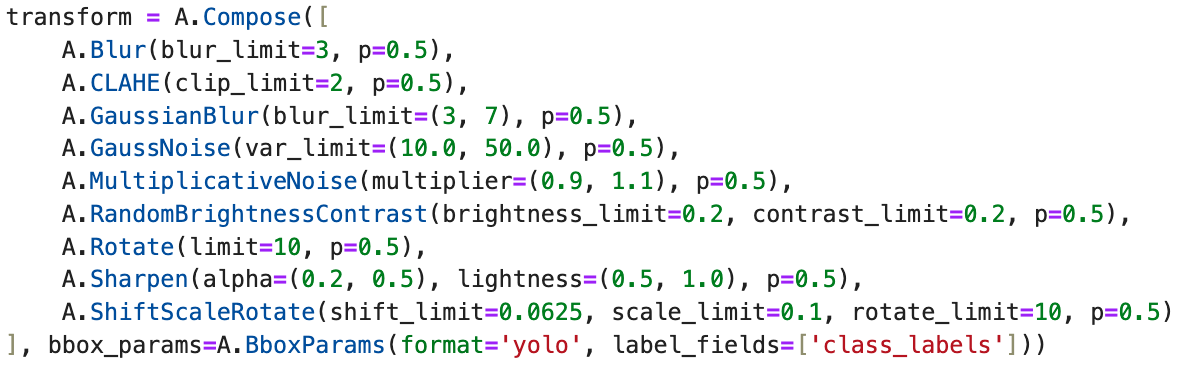
\includegraphics[width=0.9\textwidth]{files/capitoli/4-sperimentazione-risultati/assets/transform-2.png}
    \caption{\label{fig:transform-2}Definizione della nuova trasformazione di Albumentations da applicare alle immagini}
\end{figure}

Perciò, grazie allo stesso script Python utilizzato precedentemente, ho generato il dataset \texttt{augmented-data-2}.

% allungare descrivendo brevemente le trasformazioni scelte e come mai

\clearpage

\begin{figure}[ht]
    \centering
    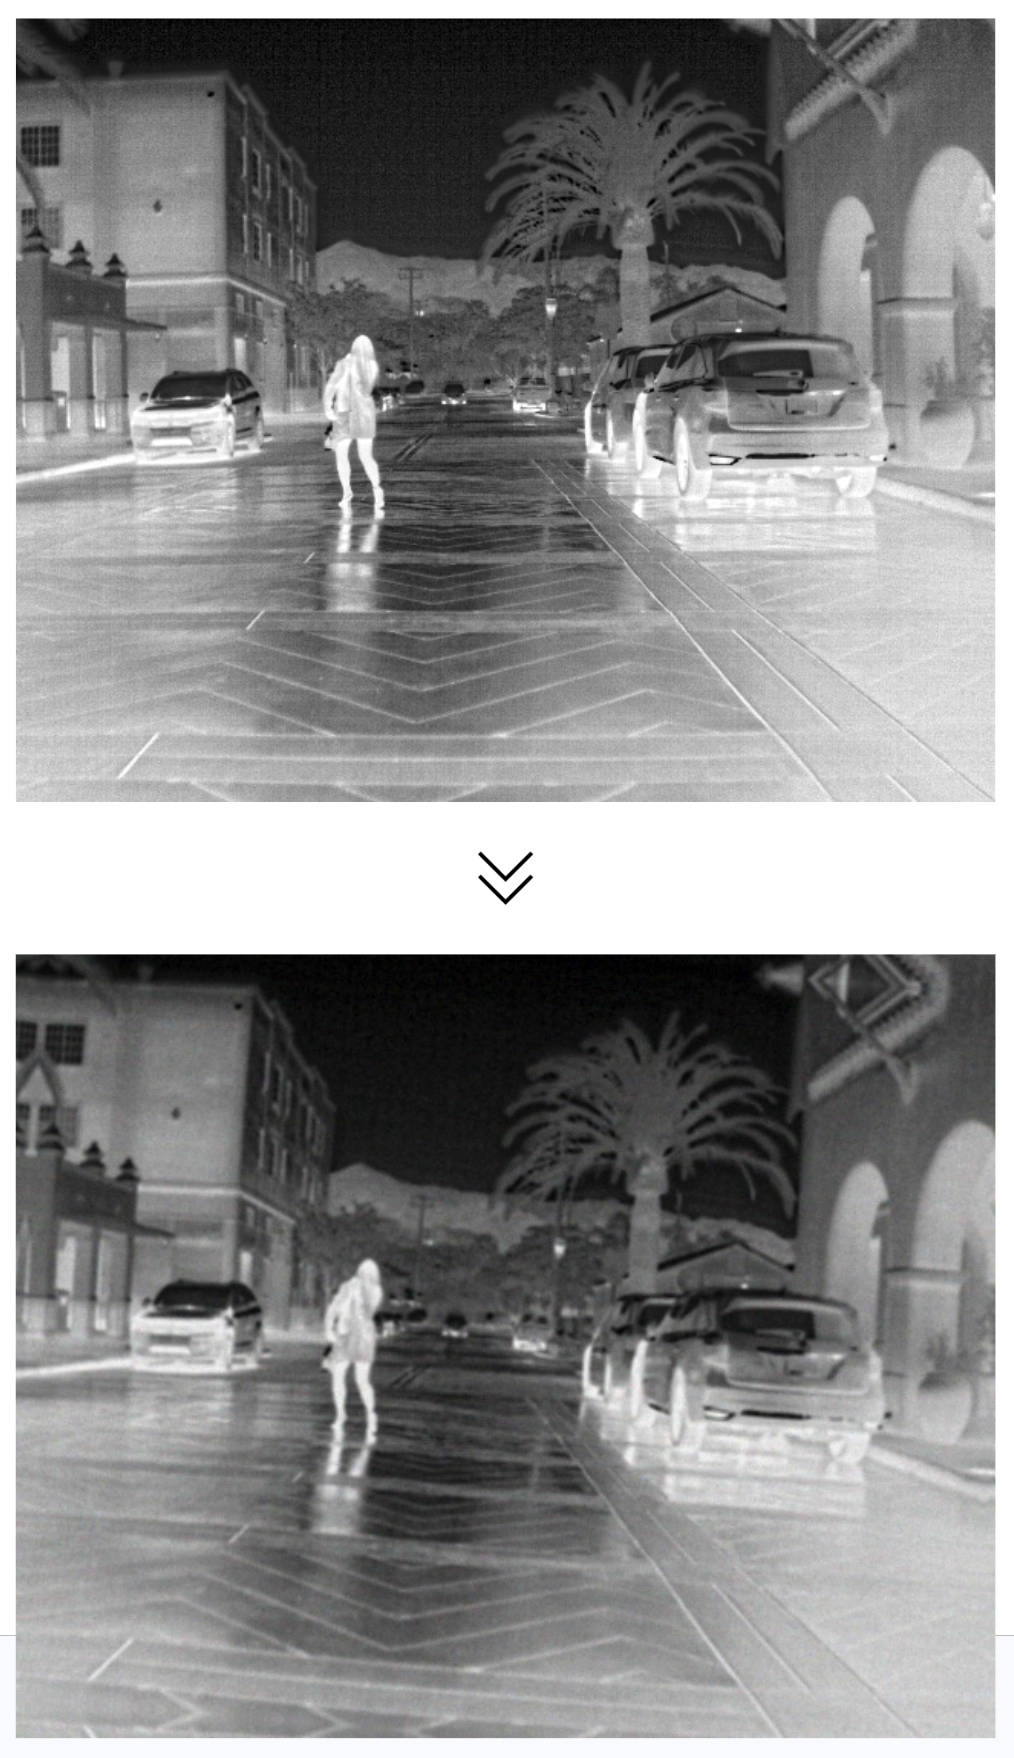
\includegraphics[width=0.8\textwidth]{files/capitoli/4-sperimentazione-risultati/assets/augmented-data-2-example.png}
    \caption{\label{fig:augmented-data-2-example}Esempio di immagine trasformata con la seconda data augmentation}
\end{figure}

\clearpage

\subsubsection{Test modelli addestrati sul secondo dataset aumentato}
A seguito del terzo addestramento, eseguito su \texttt{augmented-data-2} nelle medesime condizioni (50 epochs e batch size di 8), ho ottenuto i seguenti risultati dai test:

\begin{figure}[ht]
    \centering
    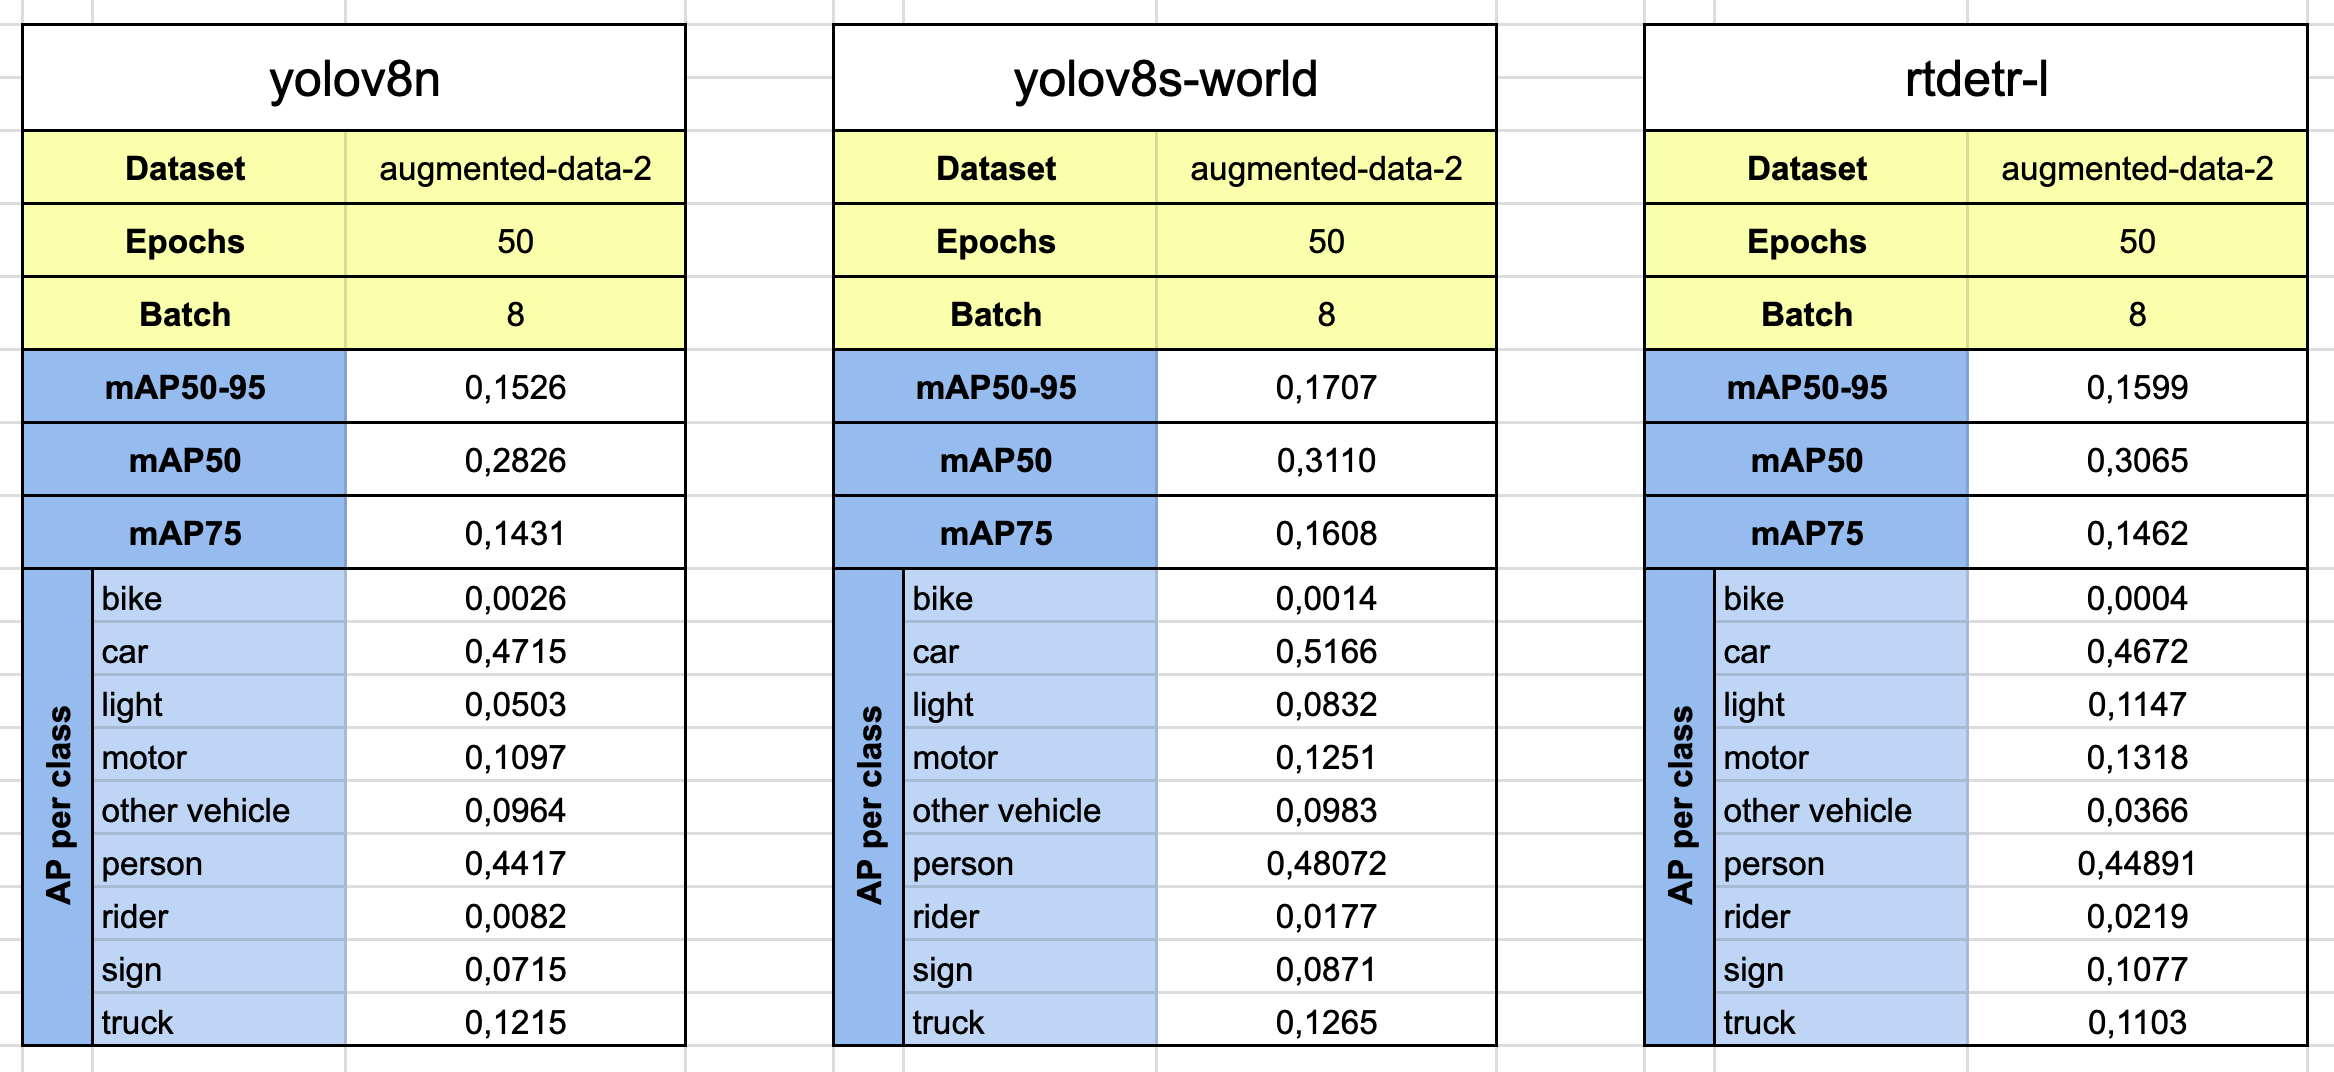
\includegraphics[width=1\textwidth]{files/capitoli/4-sperimentazione-risultati/assets/augmented-data-2-metrics.png}
    \caption{\label{fig:augmented-data-2-metrics}Risultati test dei modelli addestrati sul secondo dataset aumentato}
\end{figure}

Qua possiamo notare che i tre modelli si comportano diversamente: 

\begin{itemize}
    \item YOLOv8 ha un significativo miglioramento delle metriche rispetto ad entrambi gli addestramenti precedenti.
    \item YOLO-World ha un leggero incremento generale della mAP50-90 e della mAP50, mentre la mAP75 migliora rispetto a quella ottenuta a seguito dell fine-tuning con la prima data augmentation, ma rimane comunque inferiore a quella ottenuta con l'addestramento su dataset non aumentato.
    \item RT-DETR si comporta come nel precedente caso, mantendo tutte le metriche inferiori al primo addestramento su \texttt{filtered-data}, pur mostrando miglioramenti rispetto alla prima data augmentation.
    
\end{itemize}

\clearpage

\begin{figure}[ht]
    \centering
    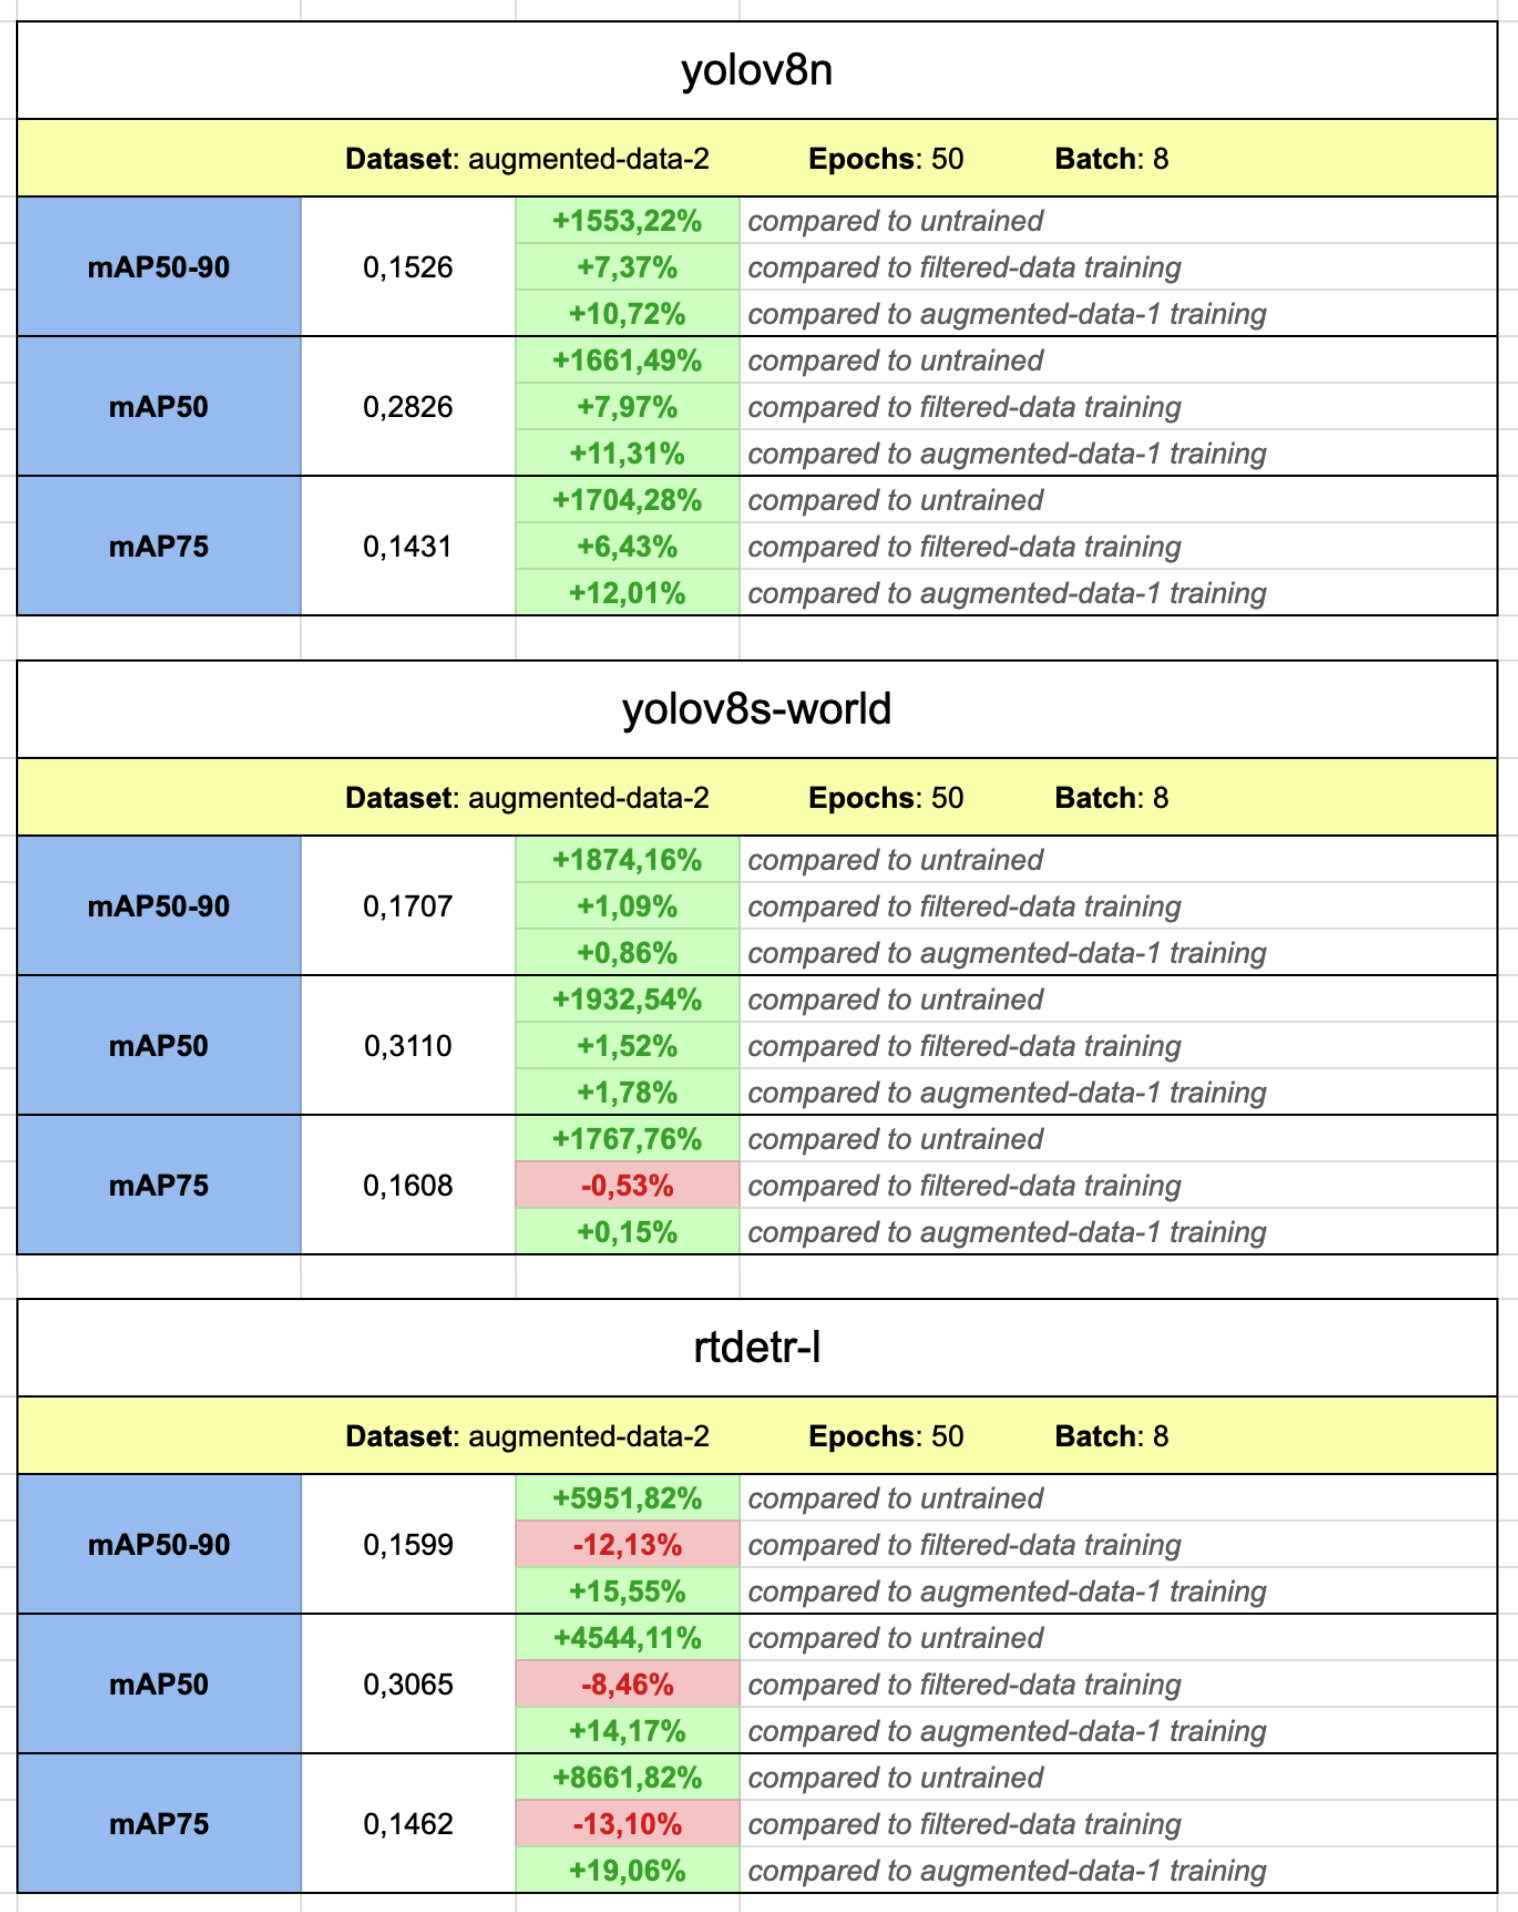
\includegraphics[width=0.9\textwidth]{files/capitoli/4-sperimentazione-risultati/assets/augmented-data-2-compare.png}
    \caption{\label{fig:augmented-data-2-compare}Confronto tra i risultati dei test dei modelli addestrati sul secondo dataset aumentato e quelli dei precedenti test}
\end{figure}

\clearpage

\begin{figure}[ht]
    \centering
    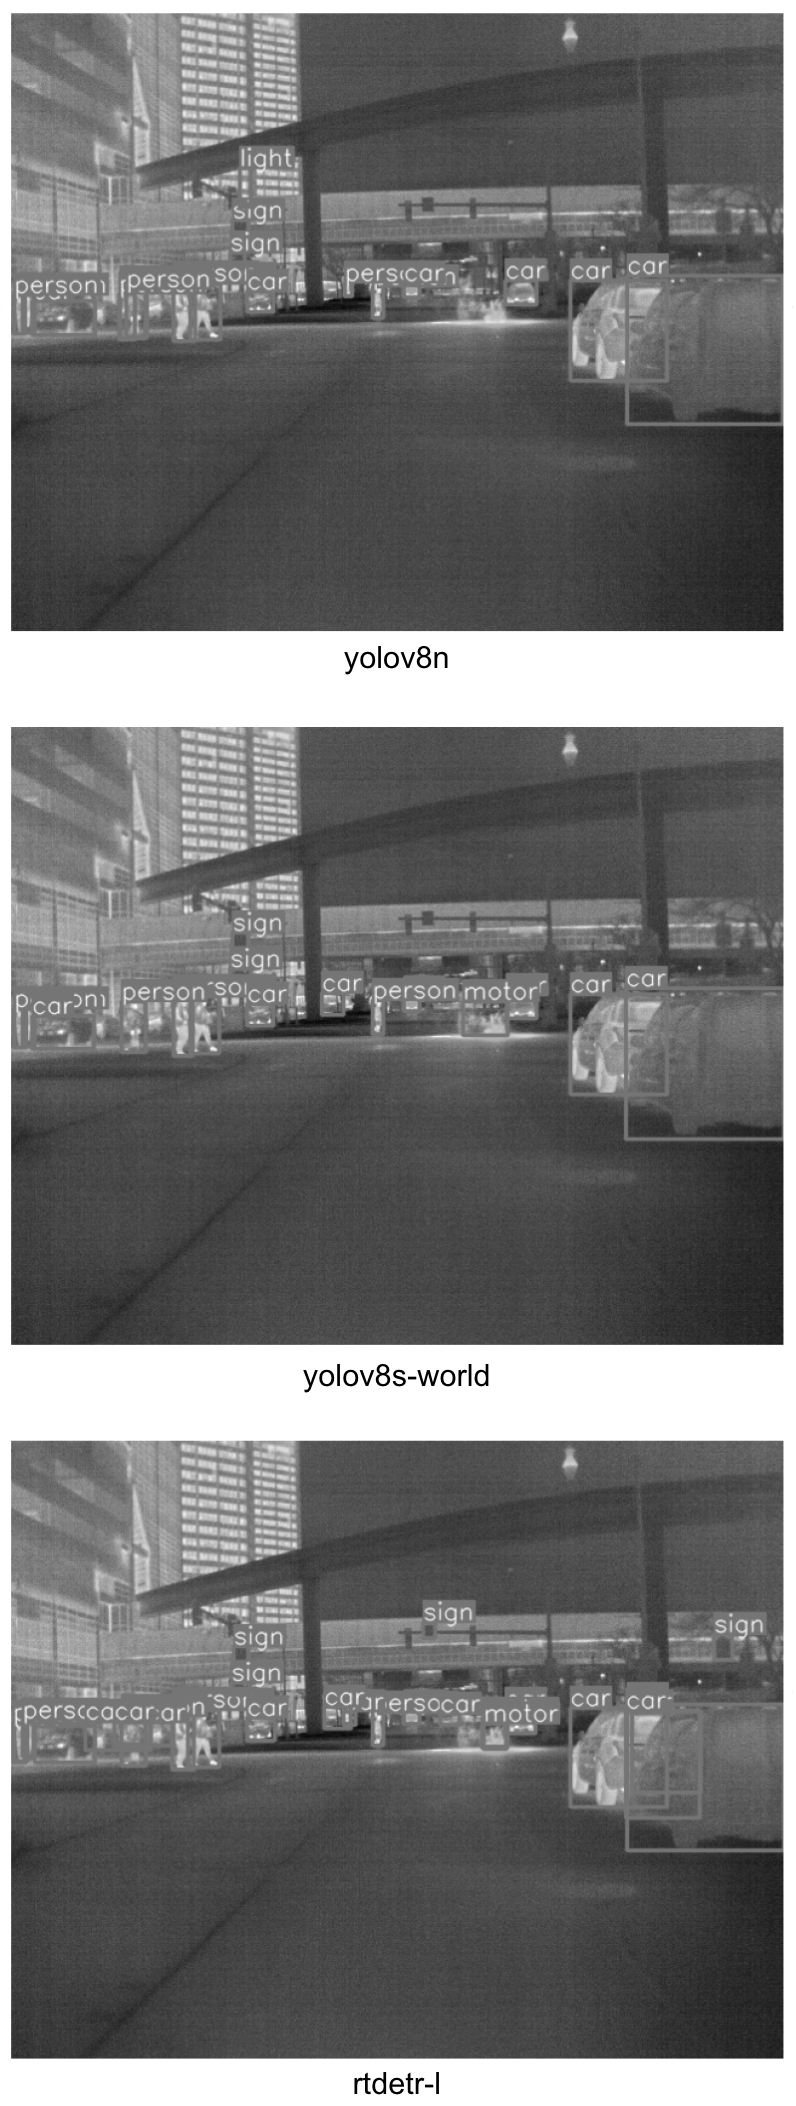
\includegraphics[width=0.6\textwidth]{files/capitoli/4-sperimentazione-risultati/assets/augmented-data-2-detections.png}
    \caption{\label{fig:augmented-data-2-detections}Detections effettutate dai modelli addestrati sul secondo dataset aumentato}
\end{figure}

\clearpage

\subsubsection{Ulteriore addestramento sul secondo dataset aumentato}
Per confermare i risultati ottenuti nei test precedenti, ho effettuato un ulteriore addestramento sul dataset \texttt{augmented-data-2}, aumentando il numero di epochs a 100. I test effettuati al termine di esso hanno prodotto i seguenti risultati:

\begin{figure}[ht]
    \centering
    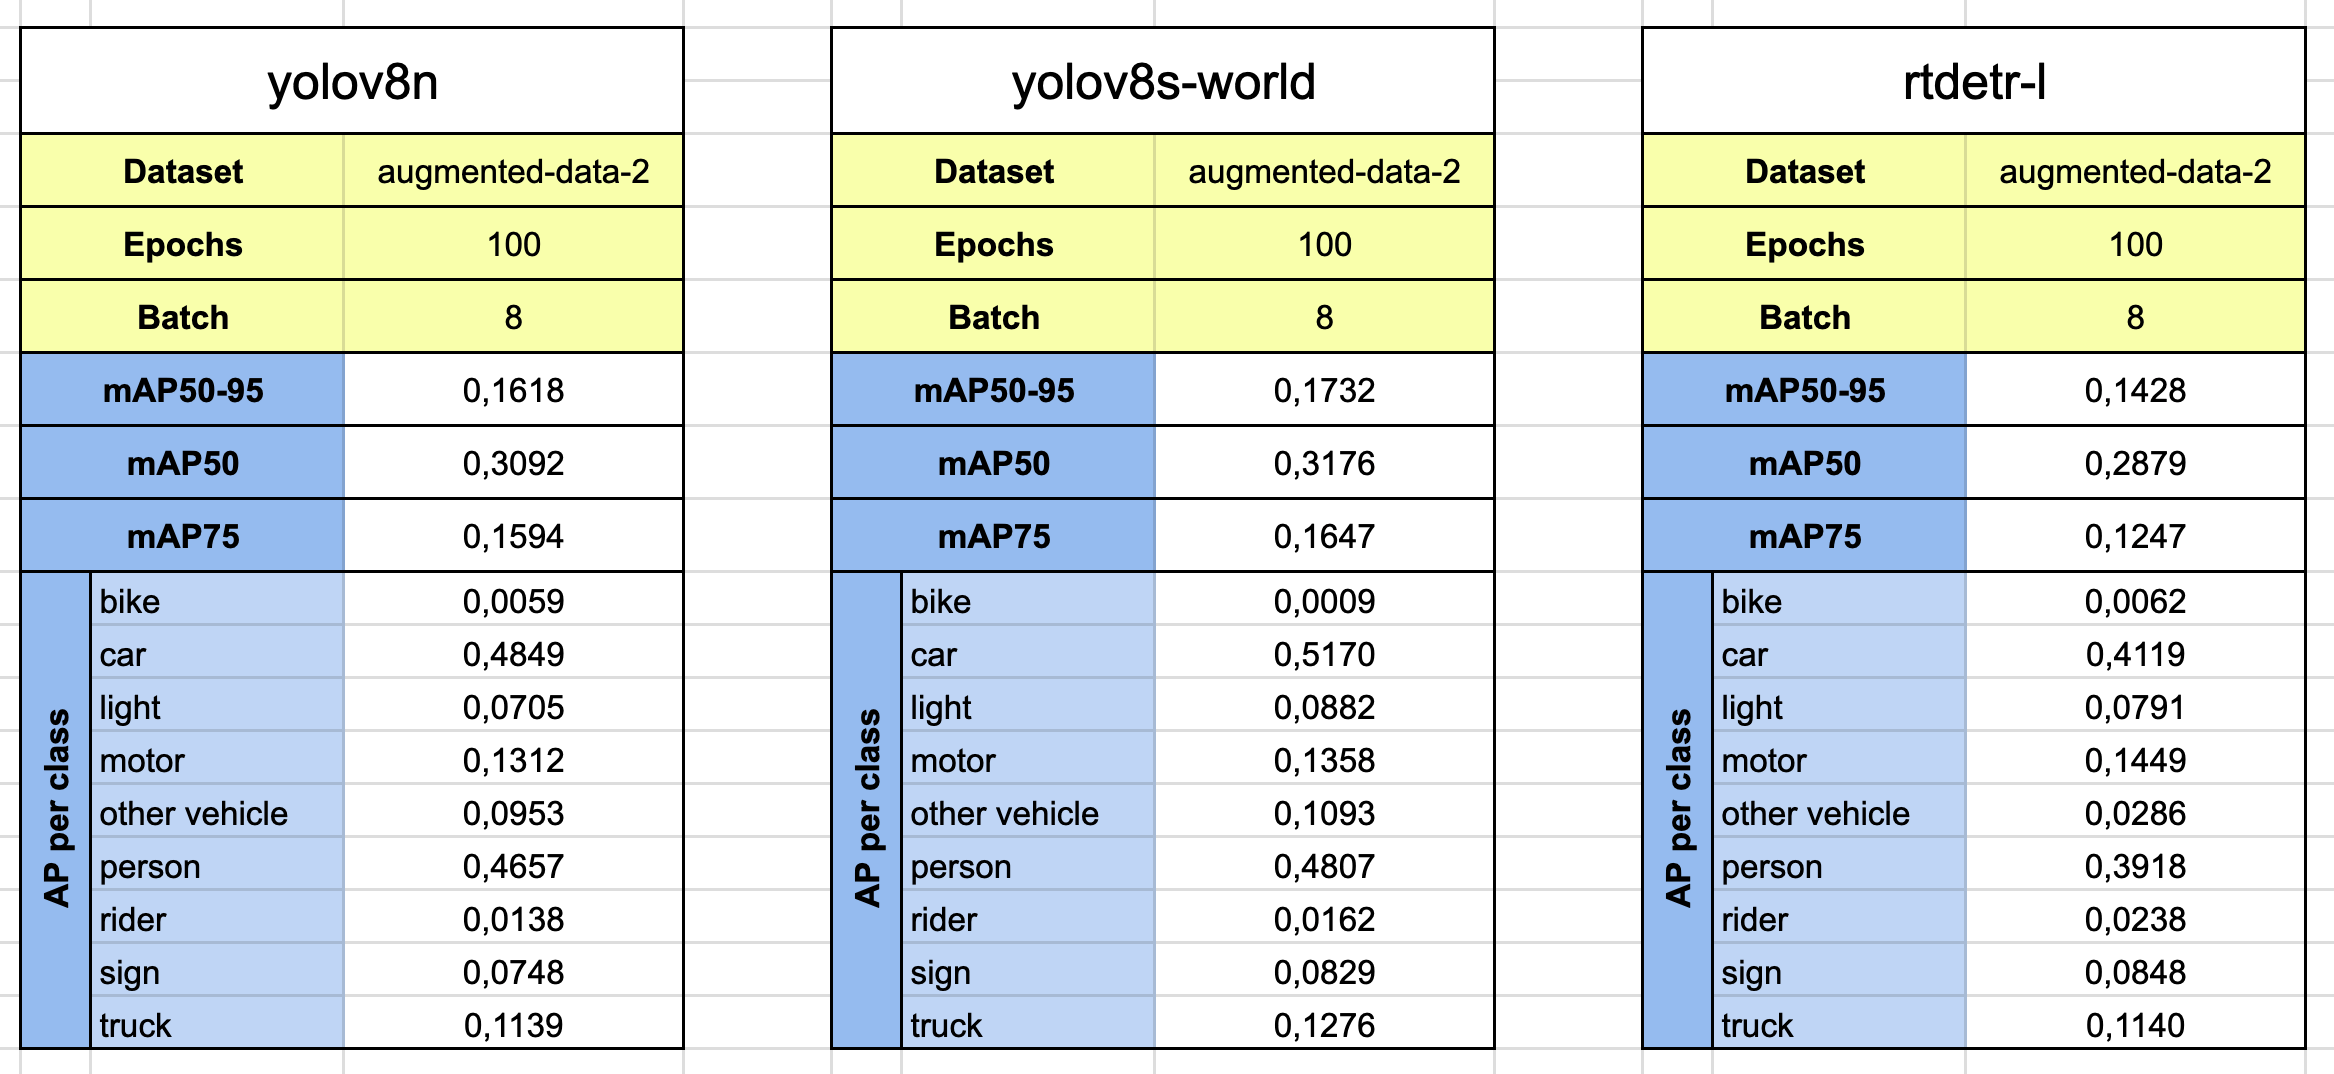
\includegraphics[width=1\textwidth]{files/capitoli/4-sperimentazione-risultati/assets/augmented-data-2(100)-metrics.png}
    \caption{\label{fig:augmented-data-2(100)-metrics}Risultati test dei modelli addestrati per 100 epochs sul secondo dataset aumentato}
\end{figure}

Dai risultati ottenuti possiamo osservare che:

\begin{itemize}
    \item YOLOv8 incrementa ulteriormente tutte le metriche di diversi punti percentuale rispetto ai precedenti addestramenti.
    \item YOLO-World incrementa tutte e tre le mAP, a differenza del precedente test in cui la mAP75 risultava inferiore a quella ottenuta con l'addestramento su \texttt{filtered-data}. Tuttavia, l'incremento è più contenuto rispetto a quello ottenuto con YOLOv8
    \item RT-DETR invece peggiora tutte le sue metriche rispetto al precedente addestramento di 50 epochs su \texttt{augmented-data-2}
\end{itemize}

\clearpage

\begin{figure}[ht]
    \centering
    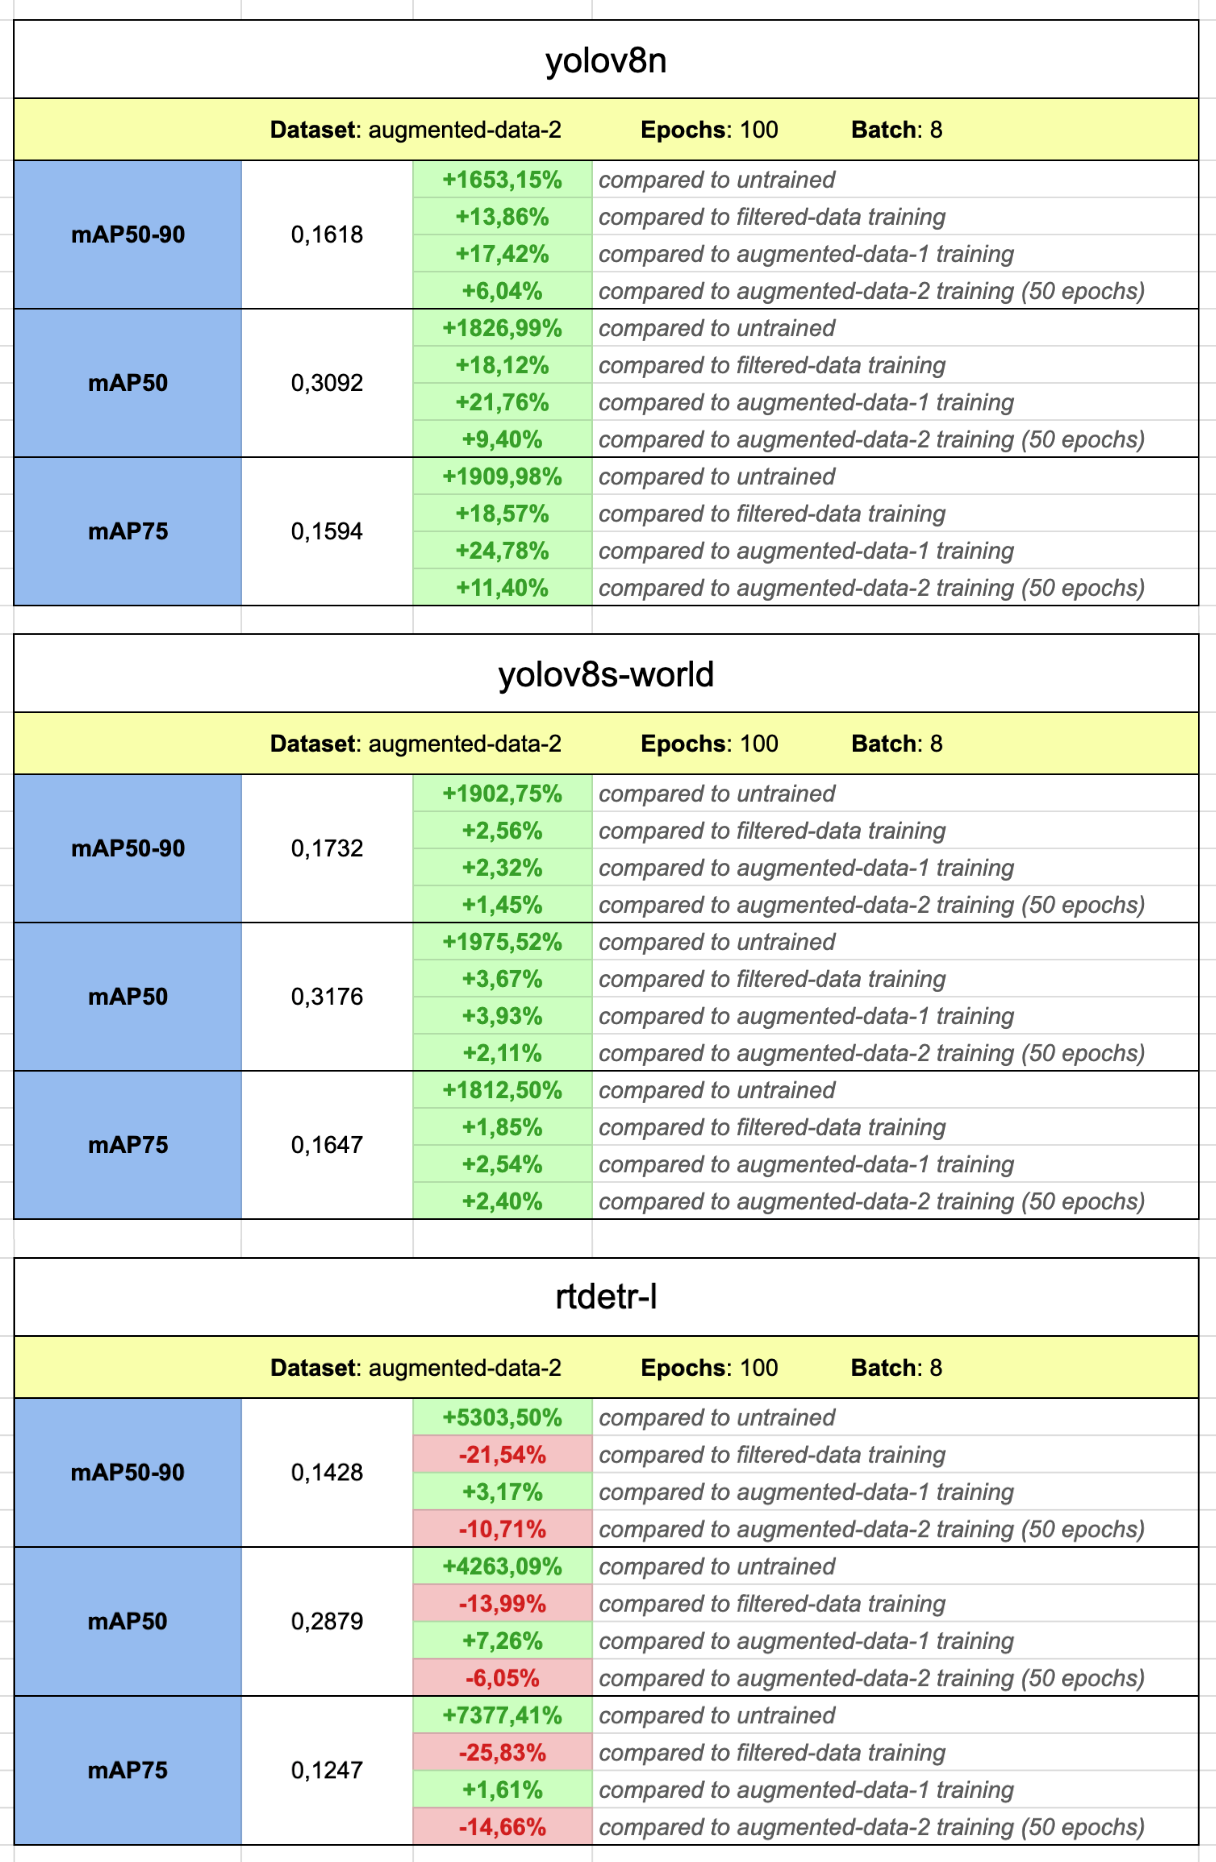
\includegraphics[width=0.9\textwidth]{files/capitoli/4-sperimentazione-risultati/assets/augmented-data-2(100)-compare.png}
    \caption{\label{fig:augmented-data-2(100)-compare}Confronto tra i risultati dei test dei modelli addestrati per 100 epochs sul secondo dataset aumentato e quelli dei precedenti test}
\end{figure}

\clearpage

\begin{figure}[ht]
    \centering
    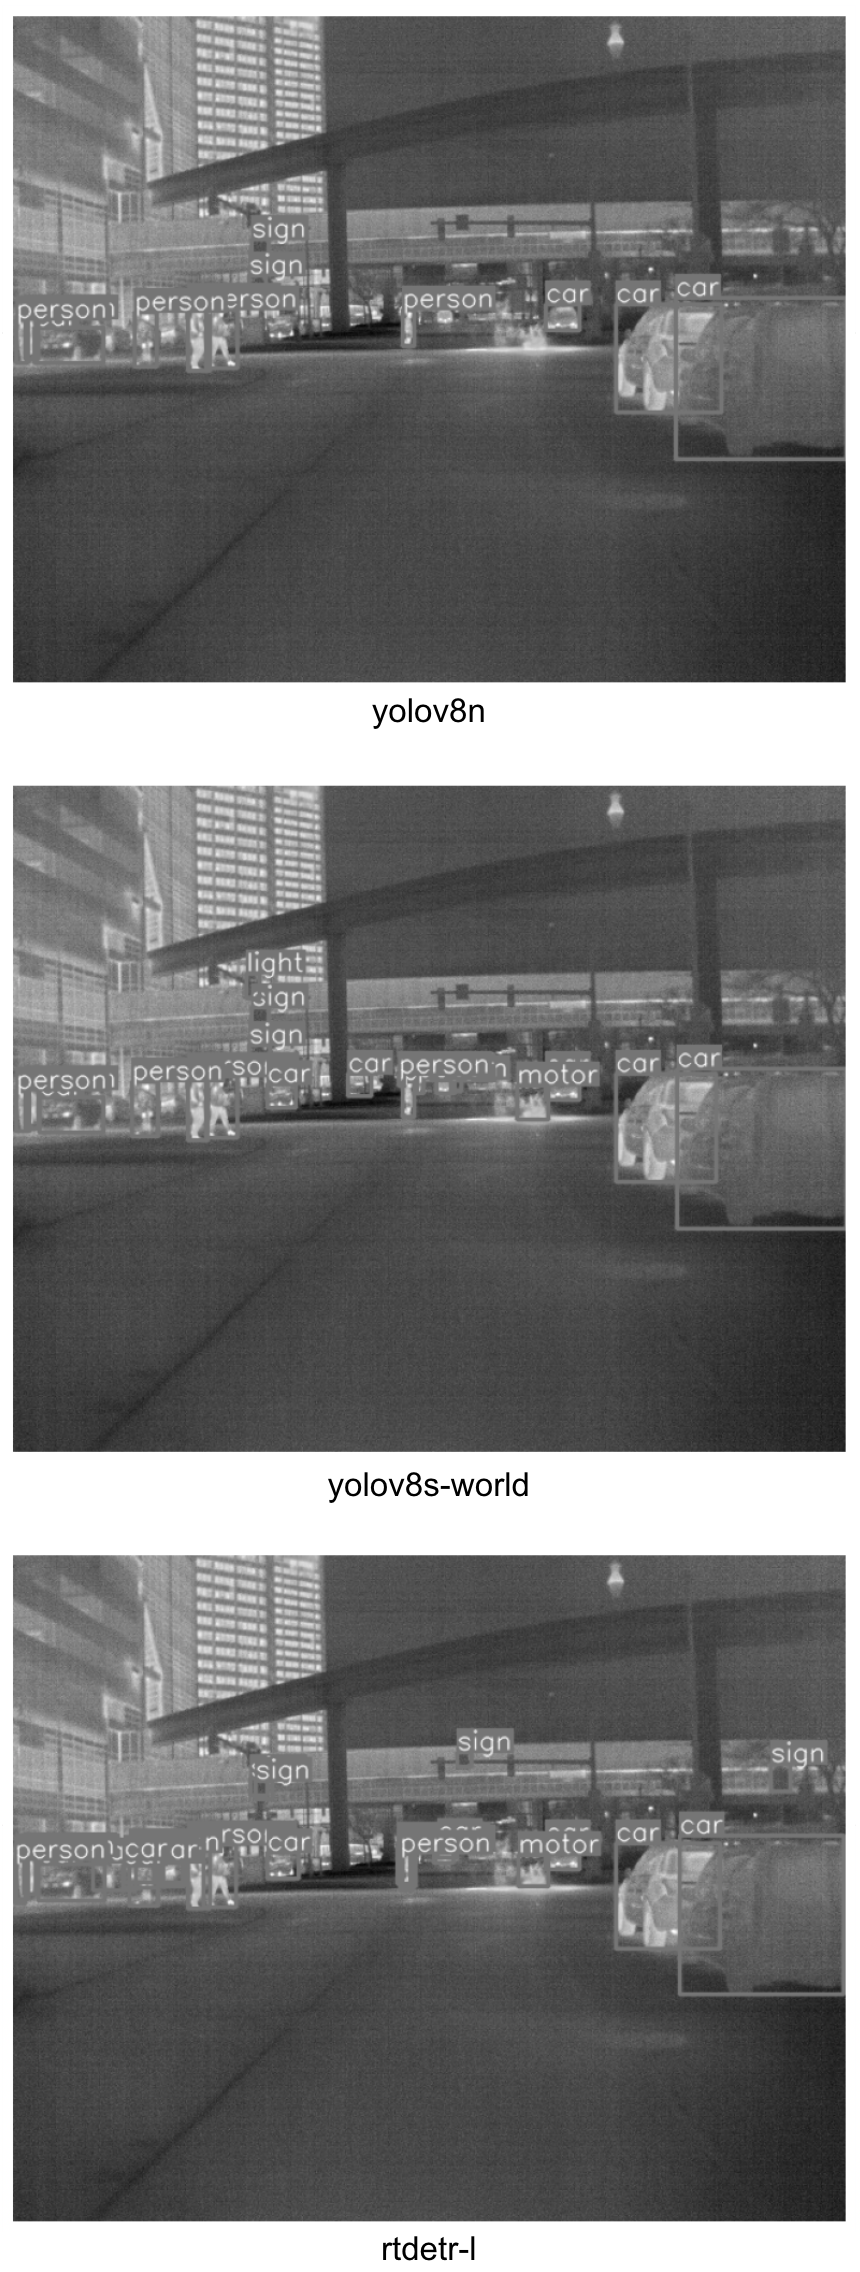
\includegraphics[width=0.6\textwidth]{files/capitoli/4-sperimentazione-risultati/assets/augmented-data-2(100)-detections.png}
    \caption{\label{fig:augmented-data-2(100)-detections}Detections effettutate dai modelli addestrati per 100 epochs sul secondo dataset aumentato}
\end{figure}

\clearpage